\documentclass{beamer}

\usepackage[ngerman]{babel}
\usepackage[utf8x]{inputenc}
\usepackage{amsmath,amsfonts,amssymb}

\usepackage[absolute,overlay]{textpos}

\newcommand{\todo}[1]{\textcolor{red}{TODO: #1}}


\usetheme{Luebeck}
\usecolortheme{orchid}

\title{Seminar Kombinatorische Optimierung: \\ Markov Random Fields}
\author{Jan Lammel}

\begin{document}
	
\frame{\titlepage}

\frame{
	\frametitle{Table of contents}
	\tableofcontents[hideallsubsections]
	
}

\section{Introduction}
\frame{
\frametitle{Introduction}

\begin{textblock}{12}(1,5)
	Until now: \\
	\begin{itemize}
	\item 2 label segmentation (foreground / background)
	\item Efficient via max-flow / min-cut
	\end{itemize}
	
	Now: \\
	\begin{itemize}
	\item Segmentation with arbitrary number of labels
	\item Actual problem is NP-complete
	\item Reduction to small 2-label problems with approximative methods
	\end{itemize}
\end{textblock}
}

\frame{
\frametitle{Introduction}
\todo{Bild + fertige Segmentierung als Motivation was am Ende rauskommen soll.}



}

\section{Mathematical problem formulation}
\subsection{Basic definitions}
\frame{
\frametitle{Basic definitions}

\begin{textblock}{14}(1, 4.5)

	\begin{itemize}
		\item Image consists of pixels $P = \{ 1, 2, ..., m \}$
		\item Segmentation labels $\mathcal{L} = \{l_1,l_ 2, ..., l_k\}$
		\item Each pixel has two statistical values
		\begin{itemize}
			\item hypothesis $f \in \mathcal{L}^m$: \ segmentation label
			\item observation $O$: \qquad \ information in the image (intensities, ...)
		\end{itemize}
	\end{itemize}
	
	\todo{Fehlt noch was wichtiges?!}

\end{textblock}

}

\subsection{Maximum a posteriori (MAP) estimate}
\frame{
\frametitle{Maximum a posteriori (MAP) estimate}

\begin{textblock}{14}(1, 4.5)

\begin{itemize}


\item Objective: $f^* = \arg \max\limits_{f} p(f|O)$ \\

\item Using Bayes' Theorem: $p(f|O) = \frac{p(O|f) p(f)}{p(O)}$ \\

\vspace{0.25cm}

Follows from definition of conditional probabilities: \\
$p(A,B) = p(A|B)p(B) = p(B|A) p(A)$ \\

\vspace{0.5cm}

\item $\Rightarrow f^* = \arg \max\limits_{f} p(O|f)p(f)$ \\

\vspace{0.4cm}

\item We need expressions for \\
	\begin{itemize}
	\item $p(O|f)$ -- \textit{likelihood} 
	\item $p(f)$ -- \textit{prior probability}
	\end{itemize}

\end{itemize}


\end{textblock}

}

\subsection{Markov Random Field (MRF)}
\frame{
\frametitle{Markov Random Fields (MRF)}

\begin{textblock}{7}(0., 4.)
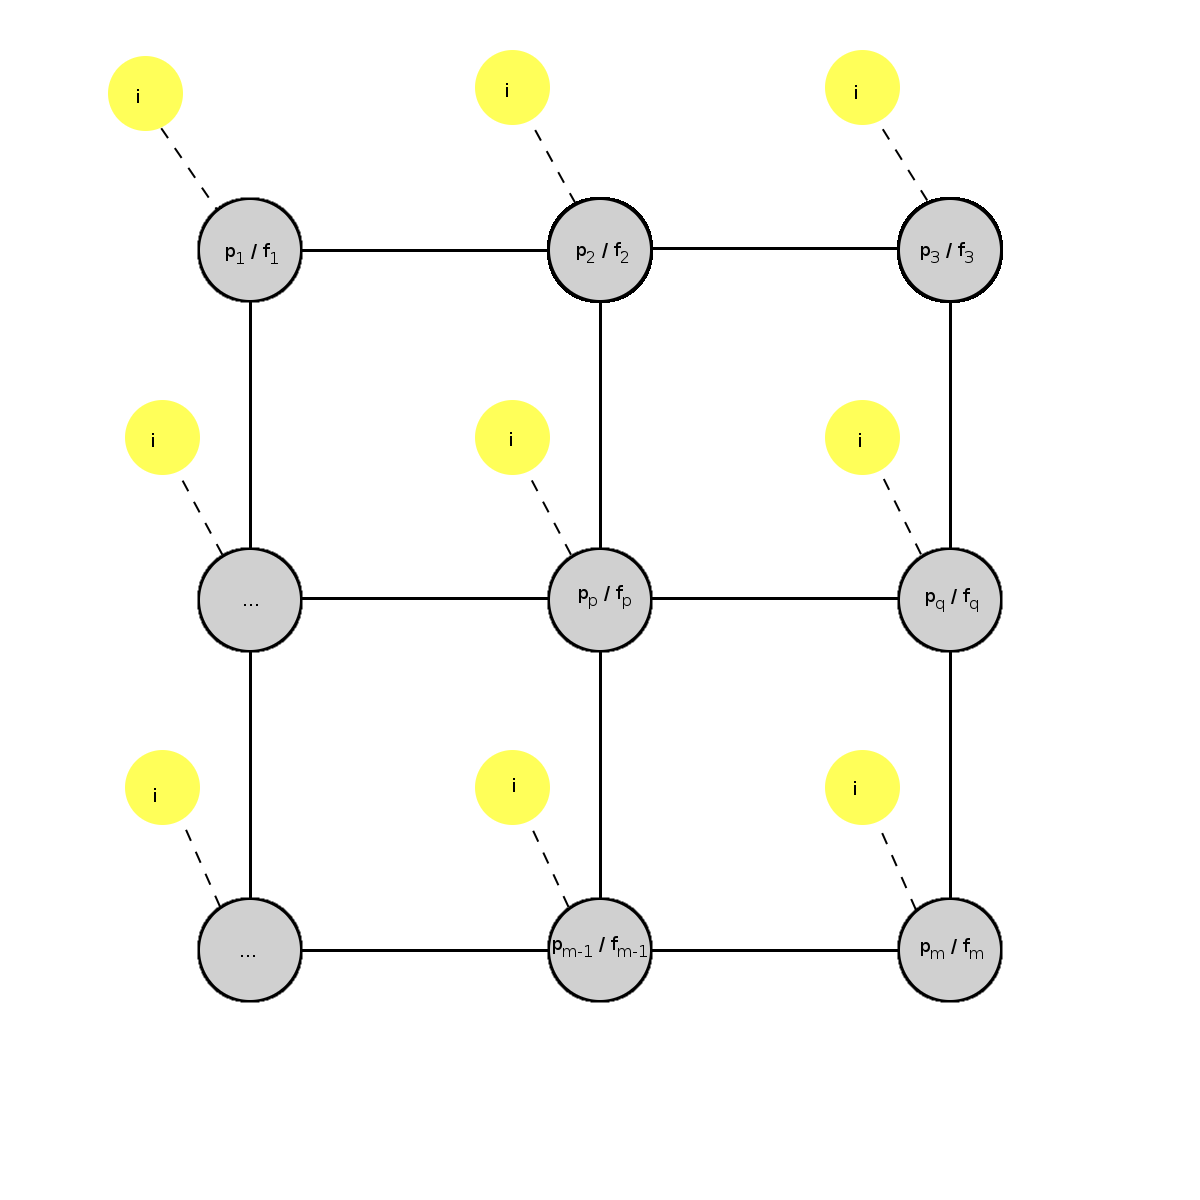
\includegraphics[width=1.15\textwidth]{/home/argo/seminar/mrf1.png}
\end{textblock}


\begin{textblock}{7}(7, 4.5)

\begin{itemize}
\item Condition for an MRF: Each random variable depends on other random variables only through its neighbors: \\

\vspace{0.25cm}

$p(f_p|f_{\mathcal{P} \setminus p}) = p(f_p|f_{\mathcal{N}_p}) $

\vspace{0.25cm}

\item here: neighborhood system are adjacent pixels

\end{itemize}

\end{textblock}

}

\frame{
\frametitle{Markov Random Fields (MRF) -- Prior term}



\begin{textblock}{7}(0., 4.)
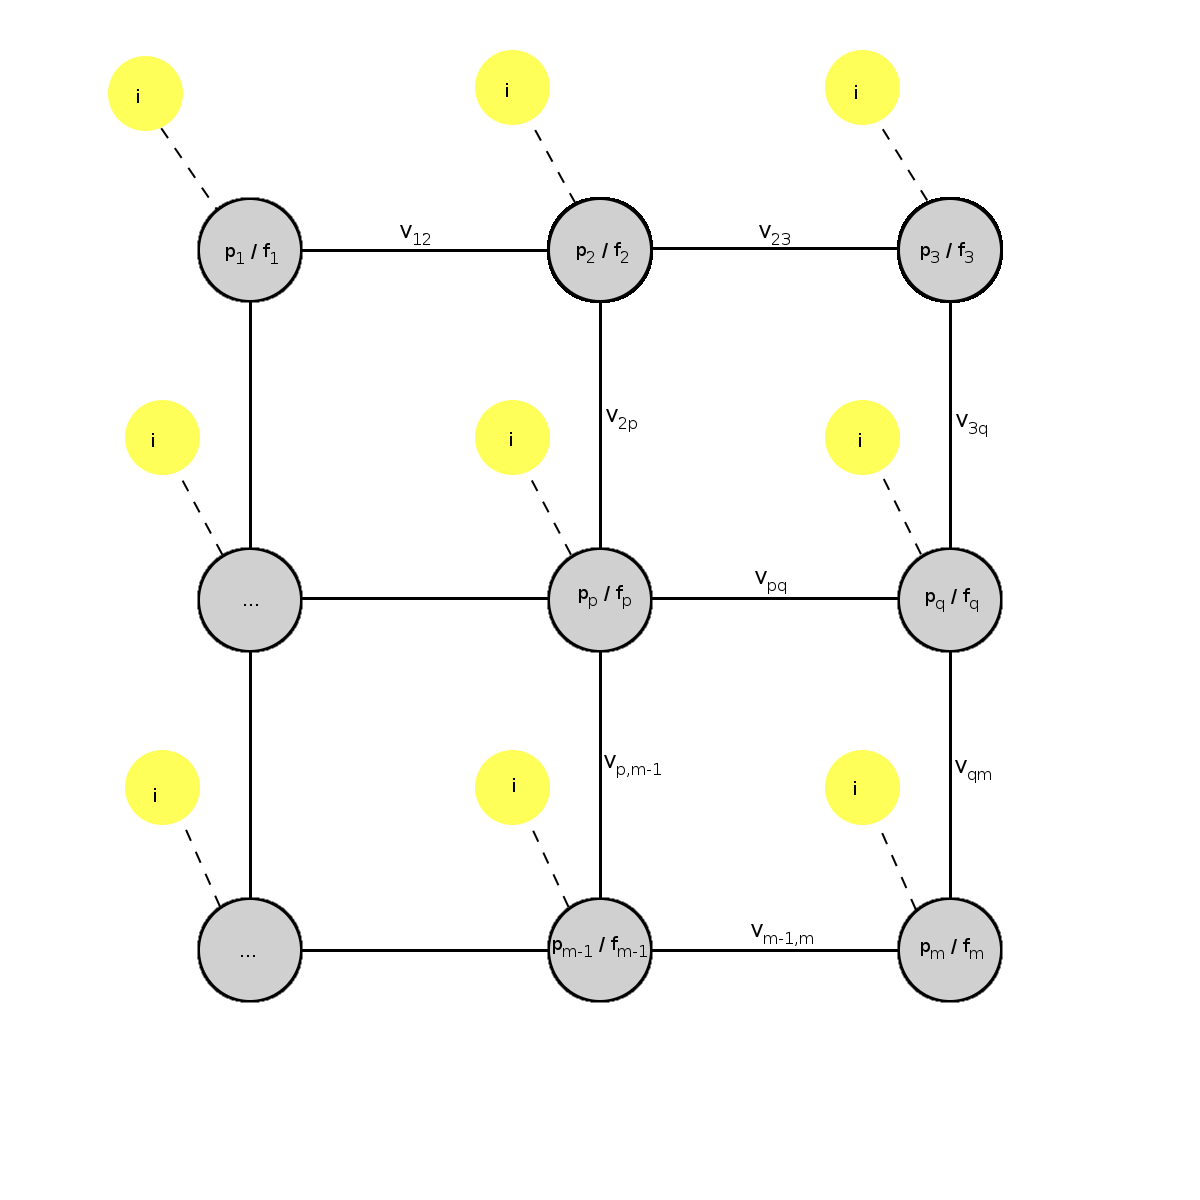
\includegraphics[width=1.15\textwidth]{/home/argo/seminar/mrf2.png}
\end{textblock}


\begin{textblock}{9}(7, 5.)

\begin{itemize}
	\item General for Markov Random Fields: \\
	Hammersley-Clifford theorem: $p(f) \propto \exp \{- \sum_C V_C(f) \}$ \\
	$C$: Clique in neighborhood system
	\vspace{0.25cm}
	\item Here: $p(f) \propto \exp\{ - \sum\limits_{p \in \mathcal{P}} \sum\limits_{q \in \mathcal{N}_p} V_{pq} (f_p, f_q) \}$
	\vspace{0.25cm}
	\item Used for smoothing to penalize different neighboring pixel labels.
\end{itemize}

\end{textblock}

}

\frame{
\frametitle{Markov Random Fields (MRF) -- Prior term}

\todo{Beispiel anhand Potts model, matrix-schreibweise}

}

\frame{
\frametitle{Markov Random Fields (MRF) -- Data term}

\begin{textblock}{7}(0., 4.)
\includegraphics[width=1.15\textwidth]{/home/argo/seminar/mrf3.png}
\end{textblock}

\begin{textblock}{9}(7, 5.)

\begin{itemize}
	\item Assume: Identical Distribution\\
	\vspace{0.2cm}
	$p(O|f) = \prod\limits_{p \in \mathcal{P}} g(i, p, f_p)$
	
	\item Example:
	\begin{equation*}
	\hspace{-0.5cm}
	g(i_p,f_p) = \begin{cases}
		\exp(-|\bar{i}_1 - i_p|) & \text{for } f_p=l_1 \\
		\exp(-|\bar{i}_2 - i_p|) & \text{for } f_p=l_2 \\
	 	\quad \vdots \\
		\exp(-|\bar{i}_k - i_p|) & \text{for } f_p=l_k \\
		\end{cases}
	\end{equation*}
	
	\vspace{0.1cm}
	$\bar{i}_l$: average intensity label $l$
\end{itemize}

\end{textblock}

}

\frame{
\frametitle{Markov Random Fields (MRF) -- Energy formulation}

\begin{textblock}{14}(1, 4)

\begin{itemize}
\item Remember objective: $f^* = \arg \max\limits_{f} p(O|f) p(f) = \arg \min\limits_{f} E(f)$ \\

\item $p(O|f) = \prod\limits_{p \in \mathcal{P}} g(i, p, f_p)$ \\
\item $p(f) \propto \exp\{ - \sum\limits_{p \in \mathcal{P}} \sum\limits_{q \in \mathcal{N}_p} V_{pq} (f_p, f_q) \}$ \\

\item Insert these expressions and take negative logarithm:
\vspace{-0.2cm}
\begin{align*}
	E(f) & = - \ln(p(O|f) p(f)) \\
	& = \sum\limits_{p \in \mathcal{P}} \sum\limits_{q \in \mathcal{N}_p} V_{pq} (f_p, f_q) - \sum\limits_{p \in \mathcal{P}} \ln(g(i, p, f_p)) \\
	& \stackrel{e.g.}{=} \sum\limits_{p \in \mathcal{P}} \sum\limits_{q \in \mathcal{N}_p} V_{pq} (f_p, f_q) + \sum\limits_{p \in \mathcal{P}} \underbrace{|\bar{i}(f_p) - i_p|}_{D_p(f_p)}
\end{align*}




\end{itemize}

\end{textblock}

}

\subsection{Multiway Cut Problem}
\frame{




}


\section{Approximative Algorithms}
\subsection{$\alpha$-$\beta$ swap}
\subsection{$\alpha$-expansion}

\section{Application example}
\subsection{flute segmentation}



	
	
	
\end{document}